\section{Scelta della camera}
Ad inizio del progetto siamo andati a lavorare con una camera \textit{SpotLight Pro Webcam}, fornita dalla casa \textit{Trust} (fig. ~\ref{fig:TrustCam}): questa camera abbiamo però visto che non era in grado di dare sufficienti garanzie di funzionamento stabile in alcune delle più comuni condizioni luminose.

Si è deciso quindi di passare ad una camera di tipo industriale, in grado di fornire delle prestazioni più \textit{stabili e affidabili}. 
La scelta è ricaduta sulla camera della casa produttrice \textit{IDS (Imaging Development System)}: si tratta del modello \textit{UI-1221LE-C-HQ} equipaggiata con la lente \textit{BM2420} della casa \textit{Lensagon}.


\begin{figure}
	\centering
	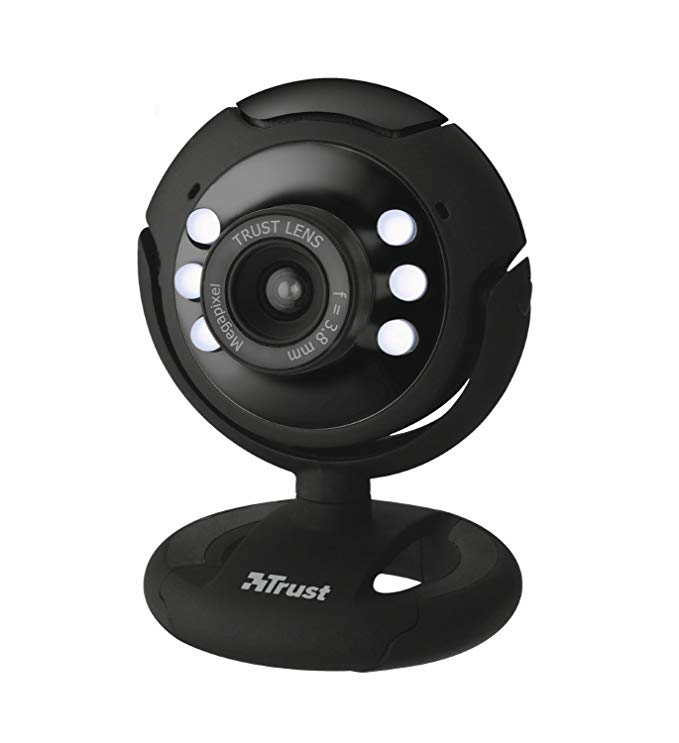
\includegraphics[width=0.5\textwidth]{Immagini/TrustCam.jpg}
	\caption{Camera utilizzata inizialmente}
	\label{fig:TrustCam}
\end{figure}


\section{Vericale o orizzontale?}
\section{Come ottenere le immagini dalla camera?}

